\begin{center}
    %%%%%%%%%%%%%%%%%%%%%%%%%%%%%%%%%
    %%%%%%%% Reactor Physics %%%%%%%%
    %%%%%%%%%%%%%%%%%%%%%%%%%%%%%%%%%
    \begin{tcolorbox}[colback=white, colframe=black, width=0.95\textwidth, arc=6pt, boxrule=1pt]
        \sectiontitle{Physics of Advanced Reactors}
        \sectioncontent{

            %% The main things in reactor physics (Olek, Zoe, Luke)
            Variance reduction methods for time-dependent Monte Carlo neutron transport.
            \par
            Updated models of DNP group parameters for Molten Salt Reactors.
            \par
            Computational modeling of flowing pebble-bed reactor systems.
            \par\vspace{1em}
        
            %% PBR images from ghastly
            \begin{minipage}{.2\linewidth}
                
\includegraphics[height = 3\textwidth]{img/ghastly1.png}
            \end{minipage}
            \hspace{.5cm}
            \begin{minipage}{.2\linewidth}
                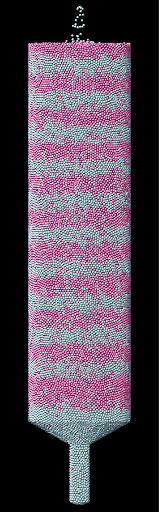
\includegraphics[height = 3\textwidth]{img/ghastly2.png}
            \end{minipage}
            \hspace{.5cm}
            \begin{minipage}{.2\linewidth}
                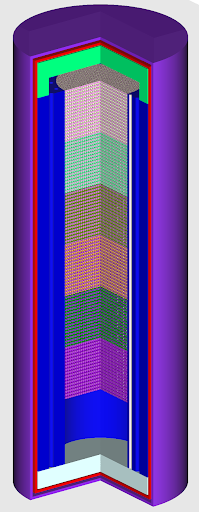
\includegraphics[height = 3\textwidth]{img/ghastly3.png}
            \end{minipage}

            \par\vspace{1em}

            \figcaption{
                Simulation of a generic pebble bed HTGR core being filled (left) and online 
                pebble recirculation (middle) using LAMMPS, and a Xe-100-like full-core 
                pebble bed HTGR (right) using SCALE \cite{richter}.
            }
        }
    \end{tcolorbox}

    %%%%%%%%%%%%%%%%%%%%%%%%%%%%%%%%%
    %%%%%%%%%% Fuel Cycles %%%%%%%%%%
    %%%%%%%%%%%%%%%%%%%%%%%%%%%%%%%%%
    \begin{tcolorbox}[colback=white, colframe=black, width=0.95\textwidth, arc=6pt, boxrule=1pt]
        \sectiontitle{Fuel Cycles and Energy System Optimization}
        \sectioncontent{
            % The main things in fuel cycle (Samar, Sam, Nathan)
            Modeling and simulating scaled isotopic consequences of deploying Accelerators Driven Systems.
            \par
            Techno-economic analysis of hybrid nuclear renewable energy systems (e.g. hydrogen microgrids).
            \par
            Fuel cycle transition scenarios for advanced reactors.
            \par\vspace{1em}

            %% Design space image from Sam
            \begin{minipage}{.7\textwidth}
                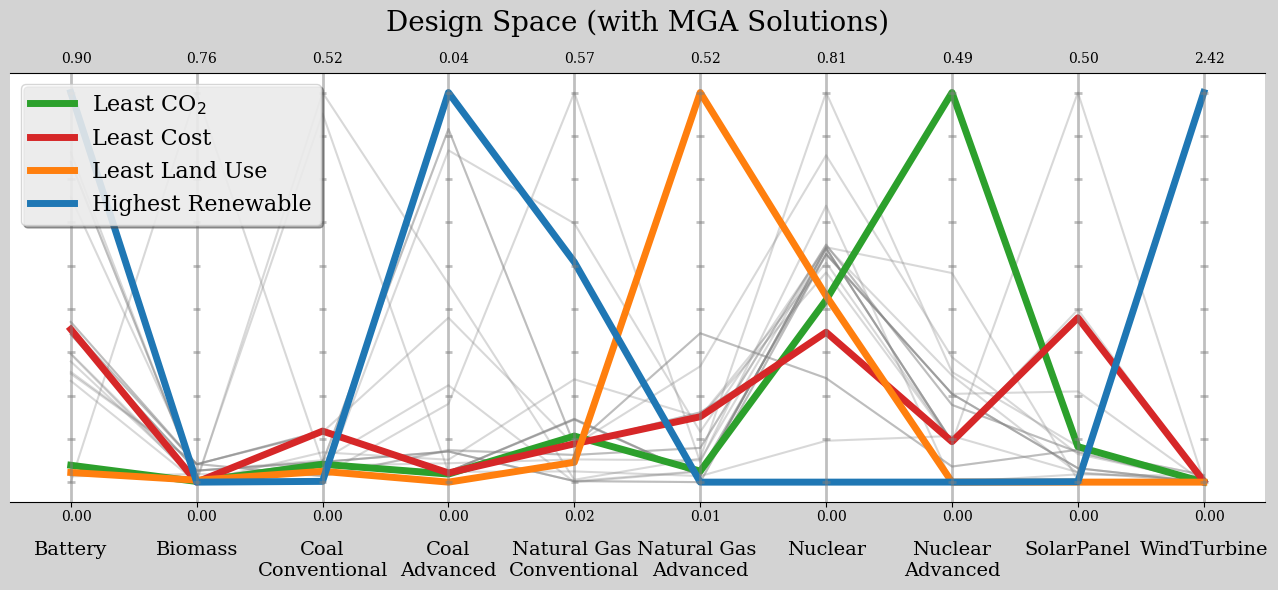
\includegraphics[width = \textwidth]{img/osier.png}
            \end{minipage}

            \par\vspace{1em}

            \figcaption{
                The design space for a four objective problem including alternative solutions suggested by MGA.
            }

            \vspace{2em}

            %% Greedy deployment image from Nathan
            \begin{minipage}{.6\textwidth}
                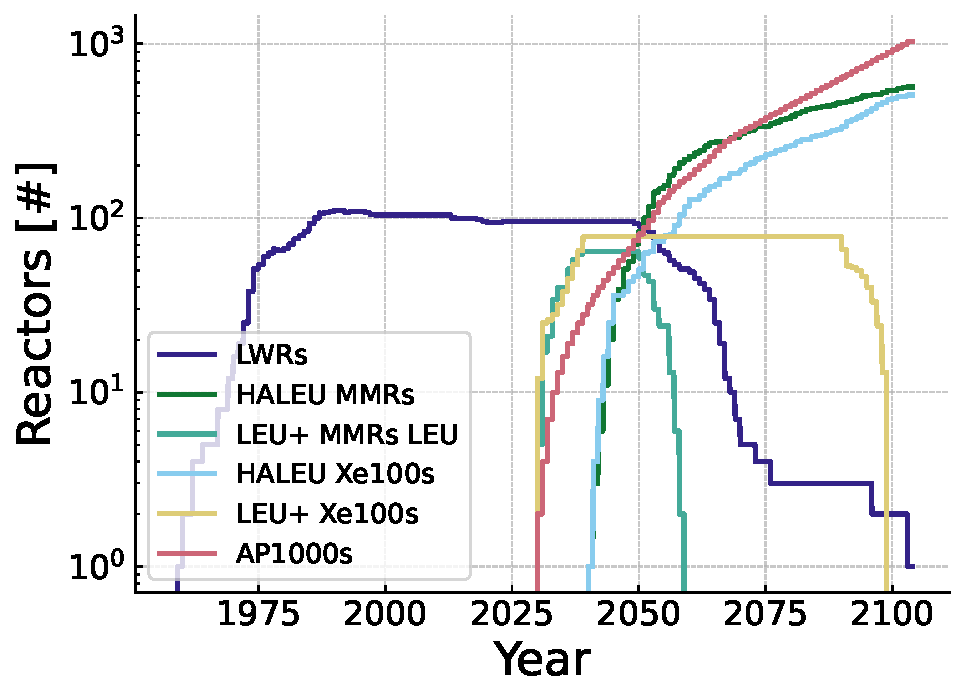
\includegraphics[width = \textwidth]{img/multi_dg2_reactors.pdf}
            \end{minipage}

            \par\vspace{1em}

            \figcaption{
                Greedy AP1000 deployment along with Xe-100s and MMRs fueled by LEU+ and HALEU fuel.
            }
        }
    \end{tcolorbox}
\end{center}